\documentclass[runningheads,a4paper]{llncs}

\usepackage[latin1]{inputenc}
\usepackage{amssymb}
\usepackage{amsmath}
\setcounter{tocdepth}{3}
\usepackage{graphicx}
\usepackage{multirow}
\usepackage{rotating}
\usepackage{subfigure}
%\usepackage{subfig}
\usepackage{url}
\usepackage{caption}

\newcommand{\keywords}[1]{\par\addvspace\baselineskip
\noindent\keywordname\enspace\ignorespaces#1}

\providecommand{\tabularnewline}{\\}

\begin{document}

\mainmatter  % start of an individual contribution

% first the title is needed
\title{Dividing chromosomes in NSGA-II island model} %TITULO PROVISIONAL

% a short form should be given in case it is too long for the running head
\titlerunning{}

% the name(s) of the author(s) follow(s) next
%
% NB: Chinese authors should write their first names(s) in front of
% their surnames. This ensures that the names appear correctly in
% the running heads and the author index.
%
\author{P. Garc\'ia-S\'anchez \and J. Ortega \and
  J. Gonz\'alez\inst{1}}
% �Se puede ayudar aqu�?
%
\authorrunning{P. Garc\'ia-S\'anchez et al.}
% (feature abused for this document to repeat the title also on left hand pages)

% the affiliations are given next; don't give your e-mail address
% unless you accept that it will be published
\institute{Dept. of Computer Architecture and Technology, University of Granada, Spain}

%
% NB: a more complex sample for affiliations and the mapping to the
% corresponding authors can be found in the file "llncs.dem"
% (search for the string "\mainmatter" where a contribution starts).
% "llncs.dem" accompanies the document class "llncs.cls".
%




\maketitle

%
%%%%%%%%%%%%%%%%%%%%%%%%%%%%%%%   ABSTRACT   %%%%%%%%%%%%%%%%%%%%%%%%%%%%%%%
%
\begin{abstract}

\keywords{Multi-objective algorithms, NSGA-II, Island model, distributed evolutionary algorithms}
\end{abstract}

%
%%%%%%%%%%%%%%%%%%%%%%%%%%%%%%%   INTRODUCTION   %%%%%%%%%%%%%%%%%%%%%%%%%%%%%%%
%
\section{Introduction}

Evolutionary Algorithms (EAs) are inherently parallelizable, as each
individual can be considered as an independent unit
\cite{Alba13parallel}, and therefore, they can improve the
computational performance over their non-parallel
versions. Multi-Objective Evolutionary Algorithms (MOEAs) are a
sub-set of... Also, as this kind of algorithms may be computationally
expensive, several parallelization methods have been proposed
\cite{Luna15Survey}. However, as MOEAs deal with whole solution sets
called Pareto Fronts (PFs), different distribution and sharing
mechanisms need to be addressed. Classic approaches, such as the
global parallel EAs (Master-Slave), or the spatially structured
algorithms (Island model or Cellullar EAs) deal with the individuals
as independent units of information, and ...  In island based models
blablabla .   % this is a lot of boilerplate - JJ

MOEAs have gained attention in the last years, mostly because their application in real-world problems. Usually these problems require a higher number of decission variables. Larger individuals require extra time for crossover, mutation and transmission. Dividing the search space...
Co-evolution model is a dimension-distributed model where a
high-dimensional problem is divided into lower dimensional problems
\cite{Gong15models}. However, usually there exist interdependences
among the elements of the solutions, so... In this paper, several of
these ideas are taken into account to compare different approaches in
chromosome division BLABLA 

The hypothesis of this paper is to demonstrate that dividing the
chromosome search space by applying crossover and mutation in
different sections in each island can improve the quality of the
solutions in the same time. %computing time? - JJ
 Two different approaches have been
compared with a baseline version of a distributed NSGA-II. Results
show that this technique can improve different quality indicators in
the same amount of time. 


%%%%%%%%%%%%%%%%%%%%%%%%%%%%%%  STATE OF THE ART  %%%%%%%%%%%%%%%%%%%%%%%%%%%%%
%
\section{State of the Art}
\label{sec:SoA}

%make it a narrative. - JJ
Distributed and parallel Evolutionary Algorithms have been used since
the early 2000s \cite{ELQUESEA} to leverage the capabilities of
clusters or grids. However, distributing MOEAs is not as easy as it is
in
single-objective EAs, as the %unfinished
. Some authors have focused in
Master-Slave approaches to parallelize MOEAs. For example, Durillo et
al. \cite{Durillo08masterslave} compared different master-slave
approaches to save time when running the EA. The method proposed by
Hiroyasu \cite{Hiroyasu07discussion} generates offspring depending of
the computation power.  

Dividing the decision or search space of EAs in different islands is
not a novel idea \cite{ALGUNOANTIGUO}. However, when using
multi-objective EAs ... 

First approaches for distributed MOEAs were studied in
\cite{Deb03distributed}. In that work, the dominance of solutions is
divided in the islands using a transformation of coordinates. Authors
concluded that dividing the search space is a good idea, but achieve
this is not trivial. Other ideas for dividing the search space include
objective separation in different processors \cite{Xiao03specialized},
or divide in two populations: one for elite and other search
\cite{Wang09parallel}. Martens, in \cite{Martens13asynchronous} used a
Barabasi-Albert island topology and selection based in migrate
individuals from a not-crowded area and acceptance based in
diversity. But the idea of dividing the decission space has been
studied in \cite{Kimovski15Parallel}. In this work, different workers
evolve sub-populations created and recombinated by a master process,
which performs different recombination alternatives from the parts by
worker processes. A high dimensional problem was used to compare these
alternatives. Although a low number of workers were used (8),
significant speedups were attained. A more similar approach to the one
presented here was studied by Dorronsoro et al. in
\cite{Dorronsoro13superlinear}. They obtained super-linear performance
BLABLABLABLA. Kimovski et al. \cite{Kimovski15Parallel} uses a
master-slave method that splits the population to several processors,
each one running in parallel a MOEA that only affects some portion of
the individuals. After certain number of generations, the master
process receive all the sub-populations to be combined. Different
combination alternatives in this step are compared. Up to 8 processors
were used in the experimental setup. However, our approach do not
broadcast all solutions to all islands for recombination, as previous
works, but only one solution to a random island, needing less
communication time. Besides, the maximum number of islands of
Dorronsoro or Kimovsky approaches was 8, while in this paper we have
used up to 128 islands. 




%
%%%%%%%%%%%%%%%%%%%%%%%%%%%%%%  METHODOLOGY  %%%%%%%%%%%%%%%%%%%%%%%%%%%%%
%
\section{Methodology and experimental setup}
\label{sec:met}



% --------------------------------------------------------------

\subsection{Baseline algorithm}

At the end of the run, all PFs of all island are aggregated in a new one and the metrics are calculated.

\subsection{Disjoint Algorithm}

In this approach, each individual of size $L$ is split into $P$ chunks of size $L/P$. Every island $p$ only performs crossover and mutation on the $p_{th}$ part of the individuals.  As in the baseline, every certain number of generations, an individual is migrated to another random island.  In the new island, this individual will be crossed and mutated as the other individuals of the island. Note that, on the contrary of another works such as \cite{EL QUE SEA} all the islands deal with complete chromosomes for fitness calculation, so our approach can deal with no decomposable problems. Figure \ref{fig:disjoint} describes this approach, with $P=5$ islands.

\begin{figure}
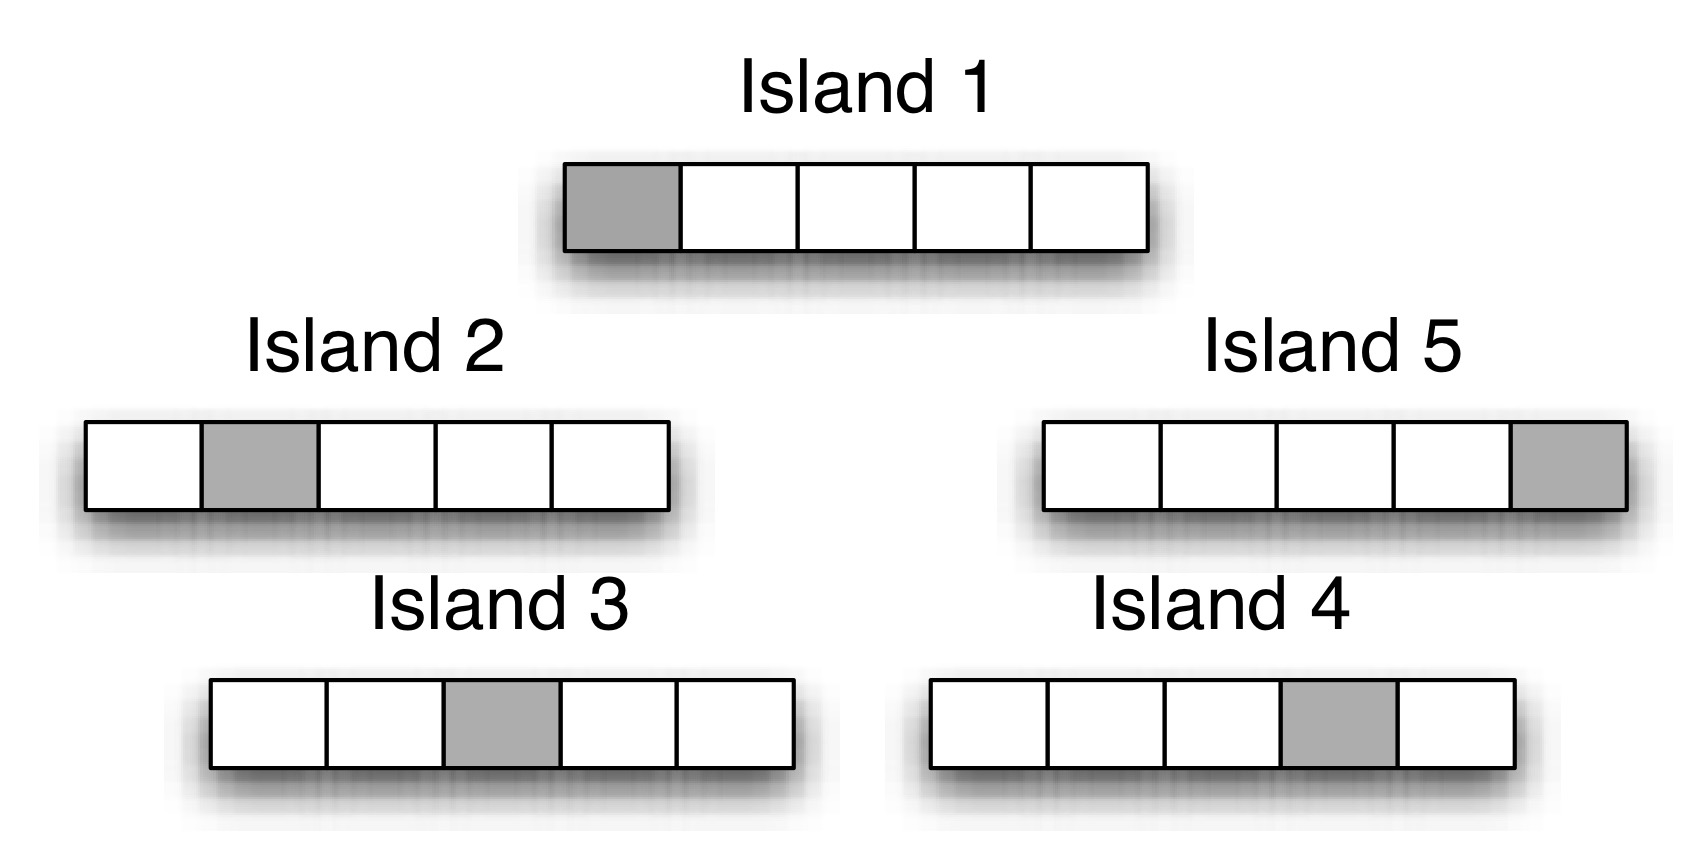
\includegraphics[width=10cm]{islandDisjoint.jpg}
\caption{Disjoint algorithm: every island $p$ only modifies the $p_{th}$ part (in grey) of the individuals.}
\end{figure}

\subsection{Overlapped Algorithm}
This approach is similar to the previous one, but every island also uses the $p+1$ and $p-1$ (module size) chunks of the individual for crossover and migration. Therefore, some kind of overlapping of the crossed and mutated parts exist between islands. Figure \ref{fig:overlapped} shows the affected parts of the individuals in each island.

 
\begin{figure}
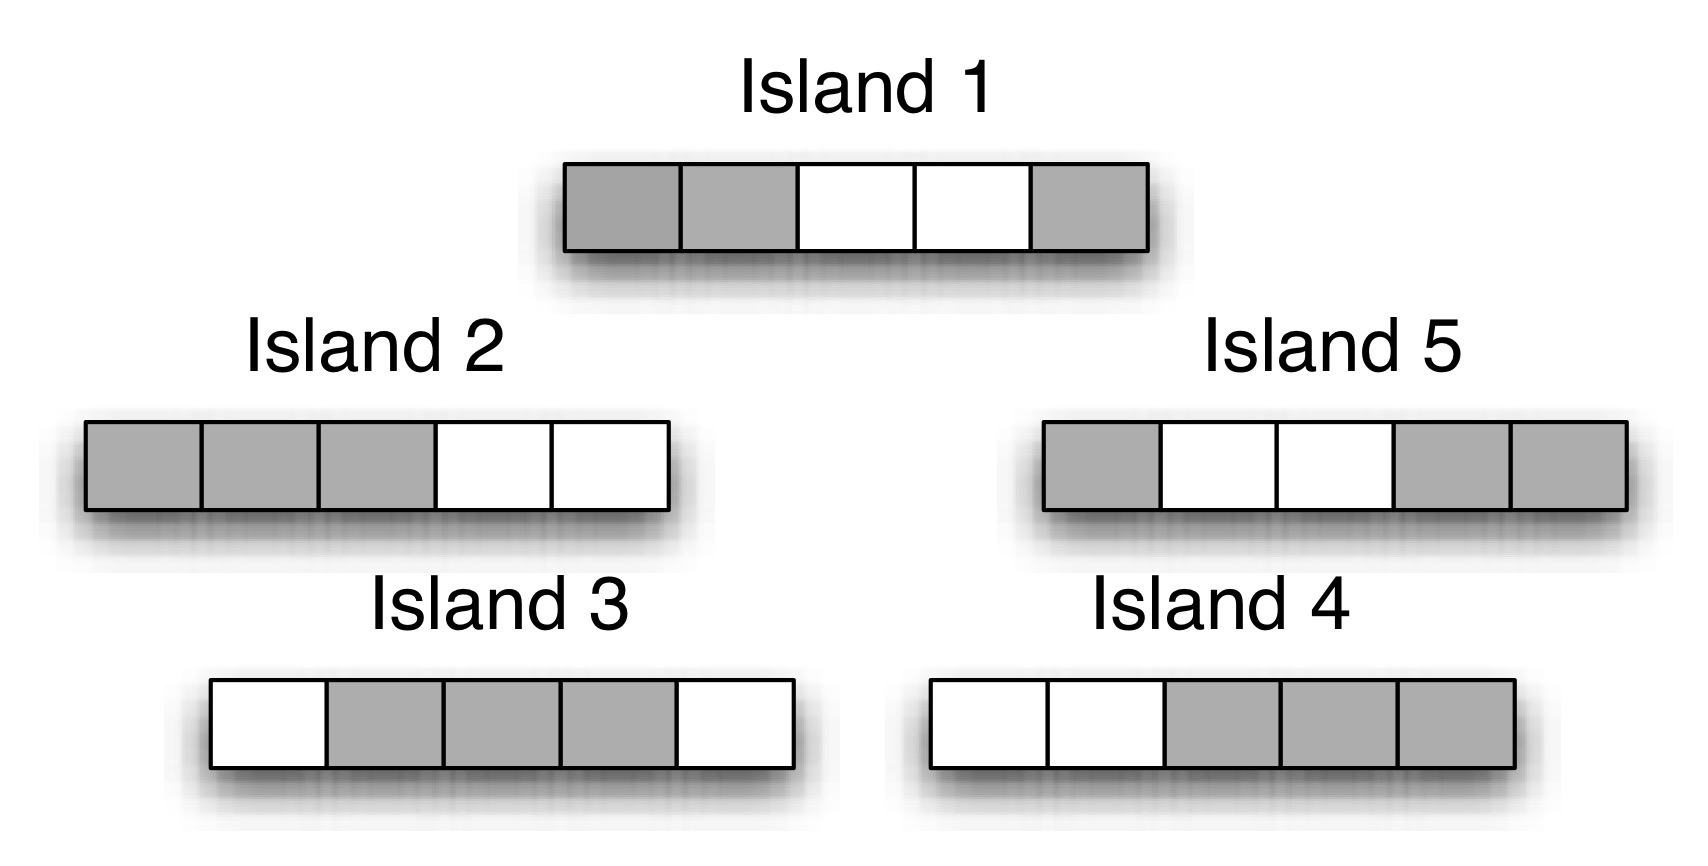
\includegraphics[width=10cm]{islandNoDisjoint.jpg}
\caption{Disjoint algorithm: every island $p$ modifies the  $p+1$, $p_{th}$ and $p-1$  parts (in grey) of the individuals.}
\end{figure}

% --------------------------------------------------------------


%%%%%%%%%%%%%%%%%%%%%%%%%%  EXPERIMENTS AND RESULTS  %%%%%%%%%%%%%%%%%%%%%%%%%%
%
\section{Experiments and Results}
\label{sec:res}

The three approaches have been launched with a different combination of chromosome lengths ($L$): 512 and 2048. Also, different number of islands ($P$) have been compared: 8, 16 and 128. This maximum number of islands have been also used in previous work in the literature \cite{Martens13asynchronous}.

The chosen problems to evaluate are the ZDT. This benchmark has been chosen because it has been previously used in different works of the literature \cite{Deb03distributed,Martens13asynchronous,Wang09parallel,Durillo08masterslave}.

Different metrics have been used to calculate the quality of the obtained PFs in each configuration.

\begin{itemize}
\item Hypervolume (HV):
\item Inverted Generational distance (IGD):
\item Spread (S):
\end{itemize}

The termination criterion used is the time. 25 seconds for dimension 512 and 100 for 2048. JUSTIFICAR

\begin{table}
\begin{center}
\begin{tabular}{|c|c|}
\hline
{\em Parameter Name} & {\em Value} \\ \hline
Number of islands ($P$) & 8, 32 and 128 \\ \hline
Chromosome size ($L$) & 512 and 2048 \\ \hline
Execution time (s) & 25000 (for 512) and 100000 (for 2048) \\ \hline \hline
Global population size ($N$) & 1024 \\ \hline
Selection type & Binary Tournament Selection \\ \hline
Replacement type & Generational \\ \hline %FERGU: tiene sentido cuando hablamos de NSGA2?
Crossover type & SBX \\ \hline
Mutation  type & Polynomial\\ \hline
Mutation probability & 1/$L$ \\ \hline
Generations between migration & 5 \\ \hline
Individuals per migration & 1 \\ \hline
Selection for migration & Binary Tournament\\ \hline
Runs per configuration & 30 \\ \hline
\end{tabular}
\caption{Parameters and operators used in the experiments.}
\label{tab:parameters}
\end{center}
\end{table}

The island model has been executed synchronously, using the ECJ Internal Island Model, in a CentOS 5.4 machine with Intel(R) Xeon(R) CPU E5520 @2.27GHz, 16 GB RAM, with Java Version 1.6.0\_16.

The ECJ framework \cite{ECJ} has been used to run the experiments. Specific operators have been developed as new modules for ECJ, and they can be downloaded from our GitHub repository under a LGPL V3 License \footnote{\url{https://github.com/hpmoon/hpmoon-islands}}.

The results are shown in Table \ref{tab:results}.

\begin{table}
\centering
\resizebox{12cm}{!}{
\begin{tabular}{|c||c|c|c||c|c|c||c|c|c||}
\hline %PON EL 0.000 a 0.0004
 
	&	\multicolumn{3}{|c|}{HV}								&	\multicolumn{3}{|c|}{Spread}								&	\multicolumn{3}{|c|}{IGD}								\\ \hline
\multicolumn{10}{|c|}{512 dimensions}																												\\ \hline
\#Islands	&	Baseline	&	Disjoint	&		Overlapped			&	Baseline	&	Disjoint		&	Overlapped			&	Baseline	&	Disjoint		&	Overlapped			\\ \hline
\multicolumn{10}{|c|}{ZDT1}																												\\ \hline
8	&	0.870	&	0.961	&		0.943			&	0.775	&	0.546		&	0.720	*		&	0.019	&	0.000		&	0.004			\\
32	&	0.803	&	0.887	&		0.957			&	0.815	&	0.837	*	&	0.621			&	0.033	&	0.014		&	0.001			\\
128	&	0.744	&	0.687	&		0.827			&	0.850	&	0.874	*	&	0.839	*		&	0.045	&	0.054		&	0.024			\\ \hline
\multicolumn{10}{|c|}{ZDT2}																												\\ \hline
8	&	0.787	&	0.919	&		0.878			&	0.913	&	0.646		&	0.907	*		&	0.035	&	0.001		&	0.011			\\
32	&	0.744	&	0.890	&		0.917			&	0.950	&	0.754		&	0.627			&	0.048	&	0.007		&	0.002			\\
128	&	0.693	&	0.592	&		0.765			&	0.971	&	0.944		&	0.917		$\bullet$	&	0.062	&	0.089		&	0.039			\\ \hline
\multicolumn{10}{|c|}{ZDT3}																												\\ \hline
8	&	0.894	&	0.976	&		0.965			&	0.895	&	0.832		&	0.922	*		&	0.012	&	0.001		&	0.003			\\
32	&	0.829	&	0.902	&		0.972			&	0.877	&	0.851		&	0.835			&	0.019	&	0.011		&	0.001			\\
128	&	0.770	&	0.726	&		0.865			&	0.891	&	0.845		&	0.845		$\bullet$	&	0.026	&	0.029		&	0.015			\\ \hline
\multicolumn{10}{|c|}{ZDT6}																												\\ \hline
8	&	0.224	&	0.503	&		0.331			&	0.992	&	1.008	*	&	0.993	*	$\bullet$	&	0.192	&	0.070		&	0.145			\\
32	&	0.192	&	0.396	&		0.454			&	0.998	&	0.998	*	&	0.980	*	$\bullet$	&	0.206	&	0.118		&	0.091			\\
128	&	0.157	&	0.114	&		0.214			&	1.004	&	0.985		&	0.979		$\bullet$	&	0.221	&	0.238		&	0.195			\\ \hline
																												
																												
																												
																												
																												
	&	\multicolumn{3}{|c|}{HV}								&	\multicolumn{3}{|c|}{Spread}								&	\multicolumn{3}{|c|}{IGD}								\\ \hline
\multicolumn{10}{|c|}{2048 dimensions}																												\\ \hline
\#Islands	&	Baseline	&	Disjoint	&		Overlapped			&	Baseline	&	Disjoint		&	Overlapped			&	Baseline	&	Disjoint		&	Overlapped			\\ \hline
\multicolumn{10}{|c|}{ZDT1}																												\\ \hline
8	&	0.754	&	0.948	&		0.889			&	0.844	&	0.587		&	0.807	*		&	0.044	&	0.003		&	0.015			\\
32	&	0.679	&	0.928	&		0.942			&	0.854	&	0.714		&	0.646			&	0.061	&	0.006		&	0.004			\\
128	&	0.660	&	0.765	&		0.907			&	0.865	&	0.860	*	&	0.802			&	0.065	&	0.036		&	0.010			\\ \hline
\multicolumn{10}{|c|}{ZDT2}																												\\ \hline
8	&	0.641	&	0.877	&		0.794			&	0.965	&	0.942		&	0.969	*	$\bullet$	&	0.078	&	0.011		&	0.033			\\
32	&	0.605	&	0.898	&		0.885		$\bullet$	&	0.980	&	0.704		&	0.755		$\bullet$	&	0.088	&	0.006		&	0.009		$\bullet$	\\
128	&	0.560	&	0.689	&		0.830			&	0.984	&	0.929		&	0.870			&	0.101	&	0.060		&	0.021			\\ \hline
\multicolumn{10}{|c|}{ZDT3}																												\\ \hline
8	&	0.773	&	0.969	&		0.922			&	0.910	&	0.865		&	0.919		$\bullet$	&	0.026	&	0.002		&	0.009			\\
32	&	0.713	&	0.937	&		0.966			&	0.903	&	0.796		&	0.839			&	0.032	&	0.007		&	0.002			\\
128	&	0.691	&	0.817	&		0.935			&	0.902	&	0.839		&	0.812		$\bullet$	&	0.035	&	0.020		&	0.007			\\ \hline
\multicolumn{10}{|c|}{ZDT6}																												\\ \hline
8	&	0.136	&	0.334	&		0.231			&	0.995	&	1.002		&	0.996	*	$\bullet$	&	0.230	&	0.144		&	0.189			\\
32	&	0.113	&	0.394	&		0.327			&	0.996	&	0.975		&	0.990	*	$\bullet$	&	0.240	&	0.118		&	0.147			\\
128	&	0.101	&	0.165	&		0.267			&	0.997	&	0.985		&	0.979		$\bullet$	&	0.245	&	0.216		&	0.172			\\ \hline


\end{tabular}
}
\caption{Quality metrics obtained after 30 runs per configuration, for the three methods compared: Baseline, Disjoint  and Overlapped. An asterisk (*) means that there is not significative difference with respect to Baseline, and a bullet ($\bullet$) indicates there is not difference beetween Disjoint and Overlapped.}
\label{tab:results}
\end{table}

Results show that... Table \ref{tab:gens} shows the generations and average solutions per island obtained in each method. 

\begin{table}
\begin{tabular}{|c||c|c|c||c|c|c||}
\hline
	&	\multicolumn{3}{|c|}{Generations}								&	\multicolumn{3}{|c|}{Avg. solutions per island}								\\ \hline
\multicolumn{7}{|c|}{512 dimensions}																			\\ \hline
\#Islands	&	Baseline	&	Disjoint	&		Overlapped			&	Baseline	&	Disjoint		&	Overlapped			\\ \hline
\multicolumn{7}{|c|}{ZDT1}																			\\ \hline
8	&	112.933	&	453.333		&	225.233			&	118.733	&	137.000		&	141.467		$\bullet$	\\
32	&	111.333	&	851.933		&	561.667			&	69.433	&	33.067		&	73.833	*		\\
128	&	126.433	&	607.200		&	606.533			&	62.367	&	18.200		&	25.567			\\ \hline
\multicolumn{7}{|c|}{ZDT2}																			\\ \hline
8	&	110.333	&	426.033		&	222.667			&	42.233	&	122.500		&	101.367			\\
32	&	113.300	&	801.800		&	595.267			&	28.800	&	26.600	*	&	62.367			\\
128	&	134.300	&	615.467		&	595.733		$\bullet$	&	20.300	&	11.433		&	13.200		$\bullet$	\\ \hline
\multicolumn{7}{|c|}{ZDT3}																			\\ \hline
8	&	106.967	&	449.533		&	227.467			&	143.933	&	138.167	*	&	160.967	*		\\
32	&	113.500	&	819.533		&	554.767			&	90.033	&	38.200		&	69.767			\\
128	&	122.633	&	630.533		&	596.300			&	70.167	&	17.933		&	25.133			\\ \hline
\multicolumn{7}{|c|}{ZDT6}																			\\ \hline
8	&	109.767	&	435.800		&	215.833			&	16.933	&	35.533		&	17.367	*		\\
32	&	113.267	&	720.233		&	518.733			&	15.800	&	11.233		&	15.100	*	$\bullet$	\\
128	&	131.333	&	597.200		&	569.500			&	15.367	&	8.467		&	8.533	 	$\bullet$	\\ \hline
																			
																			
																			
																			
																			
	&	\multicolumn{3}{|c|}{Generations}								&	\multicolumn{3}{|c|}{Avg. solutions per island}								\\ \hline
\multicolumn{7}{|c|}{512 dimensions}																			\\ \hline
\#Islands	&	Baseline	&	Disjoint	&		Overlapped			&	Baseline	&	Disjoint		&	Overlapped			\\ \hline
\multicolumn{7}{|c|}{ZDT1}																			\\ \hline
8	&	118.333	&	574.100		&	262.700			&	136.167	&	126.267		&	136.267	*	$\bullet$	\\
32	&	115.567	&	1195.800		&	721.733			&	103.867	&	35.000		&	60.267			\\
128	&	141.067	&	1266.700		&	1170.767			&	98.000	&	20.167		&	30.467			\\ \hline
\multicolumn{7}{|c|}{ZDT2}																			\\ \hline
8	&	111.833	&	584.233		&	265.933			&	32.100	&	86.600		&	78.067		$\bullet$	\\
32	&	121.367	&	1278.700		&	757.667			&	25.600	&	41.833		&	45.133		$\bullet$	\\
128	&	143.567	&	1306.700		&	1133.367			&	22.967	&	12.767		&	20.800	*		\\ \hline
\multicolumn{7}{|c|}{ZDT3}																			\\ \hline
8	&	111.700	&	589.800		&	265.567			&	167.633	&	129.333		&	144.000			\\
32	&	117.633	&	1154.133		&	772.633			&	129.167	&	36.667		&	72.767			\\
128	&	136.267	&	1379.067		&	1128.467			&	105.767	&	19.367		&	29.400			\\ \hline
\multicolumn{7}{|c|}{ZDT6}																			\\ \hline
8	&	116.867	&	585.333		&	267.133			&	22.867	&	27.267	*	&	32.600			\\
32	&	118.533	&	1082.633		&	684.500			&	22.133	&	12.067		&	16.633		$\bullet$	\\
128	&	162.267	&	1296.733		&	1102.867			&	20.167	&	7.400		&	9.267		$\bullet$	\\ \hline



\end{tabular}
\caption{Number of generations and average number of solutions per island obtained after 30 runs per configuration, for the three methods compared: Baseline , Disjoint and Overlapped. An asterisk (*) means that there is not significative difference with respect to Baseline, and a bullet ($\bullet$) indicates there is not difference beetween Disjoint and Overlapped.}
\end{table}

\section{Conclusions}


\section*{Acknowledgments} %PONER EL DEL NUEVOOOOOO!!!!
\scriptsize{This work has been supported in part by SIPESCA (Programa Operativo FEDER de Andaluc\'ia 2007-2013), TIN2011-28627-C04-02 (Spanish Ministry of Economy and Competitivity), SPIP2014-01437 (Direcci\'on General de Tr\'afico), PRY142/14 (Fundaci\'on P\'ublica Andaluza Centro de Estudios Andaluces en la IX Convocatoria de Proyectos de Investigaci\'on) and PYR-2014-17 GENIL project (CEI-BIOTIC Granada).}


%
%Hidden for double-blind review


\bibliographystyle{splncs}
\bibliography{hpmoon-evostar}


\end{document}
